\hypertarget{chap:background}{\chapter{Background}}\label{chap:background}
\section{Sentiment Analysis}
In the nutshell, sentiment analysis is to determine whether the opinion about a specific product, event, organization is positive or negative.
\subsection{The need for sentiment analysis}
Every business needs feedback from customer. Feedback help company know their product strength and weakness, drive business strategy. For example, fix the flaw in product, target new customer segment or halt a campaign. Traditional, company would survey their customer to collect feedback.  The feedback collected from direct survey are limited for many reasons, such as low population.

With the growth of social network and e-commerce, more and more people post their opinion online via blog, social network (Facebook, Twitter), e-commerce site (Amazon, eBay). Companies want to take advantage of these data. Thus, automated systems to analysis opinion are in demand.
\subsection{Different levels in sentiment analysis}
\subsubsection{Document-level}
Document-level sentiment analysis is to determine whether a document (usually a full review) about a specific entity (a product, location, service, ...) is positive or negative. For example, \cite{pang2002thumbs} perform document-level sentiment analysis on movies review data.
\subsubsection{Sentence-level}\label{sec:sent-level}
Sentence-level sentiment analysis is to determine whether a sentence expressed positive, negative. In this thesis, we focus our study on sentence-level sentiment analysis \cite{liu2012sentiment}.
\subsubsection{Aspect-level}
Aspect-level  sentiment analysis purpose is to determine opinion, whether positive or negative, against specific aspect of entity \cite{liu2012sentiment}.

\section{Feedforward neural network}
Feedforward neural network is a network whether unit in the graph does not form a cycle \cite{Goodfelloetal2016}. 

Each feedforward neural network consist at least one input layer, one output layer. Each layer contain one or more neurons (network nodes). Each neuron consist of a linear activation or non-linear activation function. 

Each node have an activation function. There are two type of activation function: Linear and non-linear. 

Example of linear function: \\
\[f(x) = Wx + b \]

Example of non-linear function: \\
\[f(x) = tanh(x) \]
\[f(x) =\frac{1}{1+e^{-x}} \]

\subsection{Single-layer perceptron}
Singlelayer perceptron is a feedforward neural network only have one input layer and one output layer of neuron unit (See fig \ref{fig:singleperceptron}). Singlelayer perceptron cannot solve some problem such as XOR.
\begin{figure}[H]
	\centering
	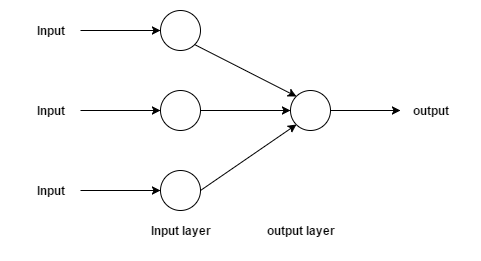
\includegraphics[width=0.7\linewidth]{../figure/singleperceptron}
	\caption[Single-layer Perceptron]{Single-layer Perceptron}
	\label{fig:singleperceptron}
\end{figure}



\subsection{Multi-layer perceptron}
Multilayer perceptron (MLP) is a feedforward neural network consist of 2 or more layer (See fig \ref{fig:multilayerperceptron}). First layer called input layer. Last layer called output layer. All layer between input and output layer are hidden layer. A series of linear function is equal to 2 layer perceptron. Hence, MLP always contain non-linear activation function. In MLP, every unit of previous layer connect to all unit in next layer.

\begin{figure}[H]
	\centering
	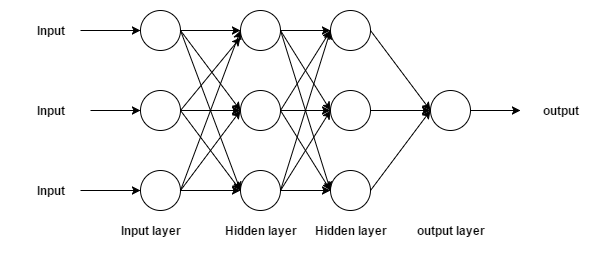
\includegraphics[width=0.7\linewidth]{../figure/multilayerperceptron}
	\caption[Multi-layer Perceptron]{Multi-layer Perceptron}
	\label{fig:multilayerperceptron}
\end{figure}

\subsection{Forward pass}
Forward pass, or forward propagation, is a process which information from input x flow through the network to output y. In MLP forward pass, an input x is feed through first layer, also known as input layer. Output from first layer is use as input for second layer, and so on until it reach last layer, output layer. Output from output layer are output of MLP. 

For example: a MLP with 4 activation function: $f(x)$, $g(x)$, $h(x)$, $k(x)$. With $f(x)$ is input layer, $k(x)$ is output layer, and $g(x), h(x)$ are hidden layers .With input $x$, then MLP has output $ y = k(h(g(f(x))))$.

\subsection{Cost function}
Cost function $J(\theta)$  is a measurement how far predicted  $\hat y$ from expected label $y$. When our model predict exactly the labeled output, then cost function is zero. The problem is to minimize the cost function. Cost function of MLP dependent on output layer.

For most of our experiment, we would use softmax output layer and cross-entropy loss function.
\subsection{Backward pass}





\section{Parse tree in NLP}
Parse tree is a syntactic representation of a sentence. In this thesis, we work on two type of parse tree, Constituency Parse Tree, and Dependency Parse Tree.
\subsection{Constituency Parse Tree}
Constituency Parser breaks sentences into smaller phases. The root node represents a sentence. Children node represent a phrase or word constitutes parent node. Each leaf node contains a word or a punctuation. Each inner node contains a phrase. Each node is Part-of-speech tag labeled. Edges are unlabeled.

Constituency Parse Tree are construct based on Chomsky Phase Structure \cite{chomsky2002syntactic}. Given a list of rule, derive sentences following the rule. Constituency Parse Tree illustrates the derivation.


% \begin{equation}
% \label{eq:crule}
% \begin{aligned}
% &S \leftarrow NP + VP + .  \\
% &NP \leftarrow PRP  \\
% &NP \leftarrow DT + NN  \\
% &VP \leftarrow VBP + NP\\
% &VRP \leftarrow I \\
% &DT \leftarrow the \\
% &NN \leftarrow cat \\
% &VBP \leftarrow feed \\
% \end{aligned}
% \end{equation}
For example, we have the following rule:
\begin{enumerate}[label=(\roman*)]
    \item $S \leftarrow NP + VP + .$
    \item $NP \leftarrow PRP $
    \item $NP \leftarrow DT + NN$
    \item $VP \leftarrow VBP + NP$
    \item $VRP \leftarrow I$
    \item $DT \leftarrow the$
    \item $NN \leftarrow cat$
    \item $VBP \leftarrow feed$
\end{enumerate}
We apply rule to "I feed the cat". Result of derivation in Table \ref{ifeedmycat}  where roman on right column indicate the rule is use to derive previous statement. The derivation is illustrate in fig \ref{fig:ifeedthecatconstituency}

% \begin{equation}
% \label{eq:catparse}
% \begin{aligned}
% &S \\
% &NP + VP + .\\
% & PRP + VP + . \\
% & PRP + VBP + NP + . \\
% & PRP + VBP + DT + NN + . \\
% & I + VBP + DT + NN + . \\
% & I + feed + DT + NN + . \\
% & I + feed + my + NN + . \\
% & I + feed + my + cat + . \\
% \end{aligned}
% \end{equation}

\begin{table}[H]
	\centering
	\begin{tabular}{ll}
	S	&  \\
	NP + VP + .	& (i) \\
	PRP + VP + .	& (ii) \\
	PRP + VBP + NP + .	& (iv)  \\
	PRP + VBP + DT + NN + .	& (iii) \\
	I + VBP + DT + NN + .	&  (v) \\
	I + feed + DT + NN + .	&  (viii) \\
	I + feed + the + NN + .	&  (vi) \\
	I + feed + the + cat + .	& (vii)
	\end{tabular}
\caption{I feed the cat derivation}
\label{ifeedmycat}
\end{table}

\begin{figure}[H]
    \centering
    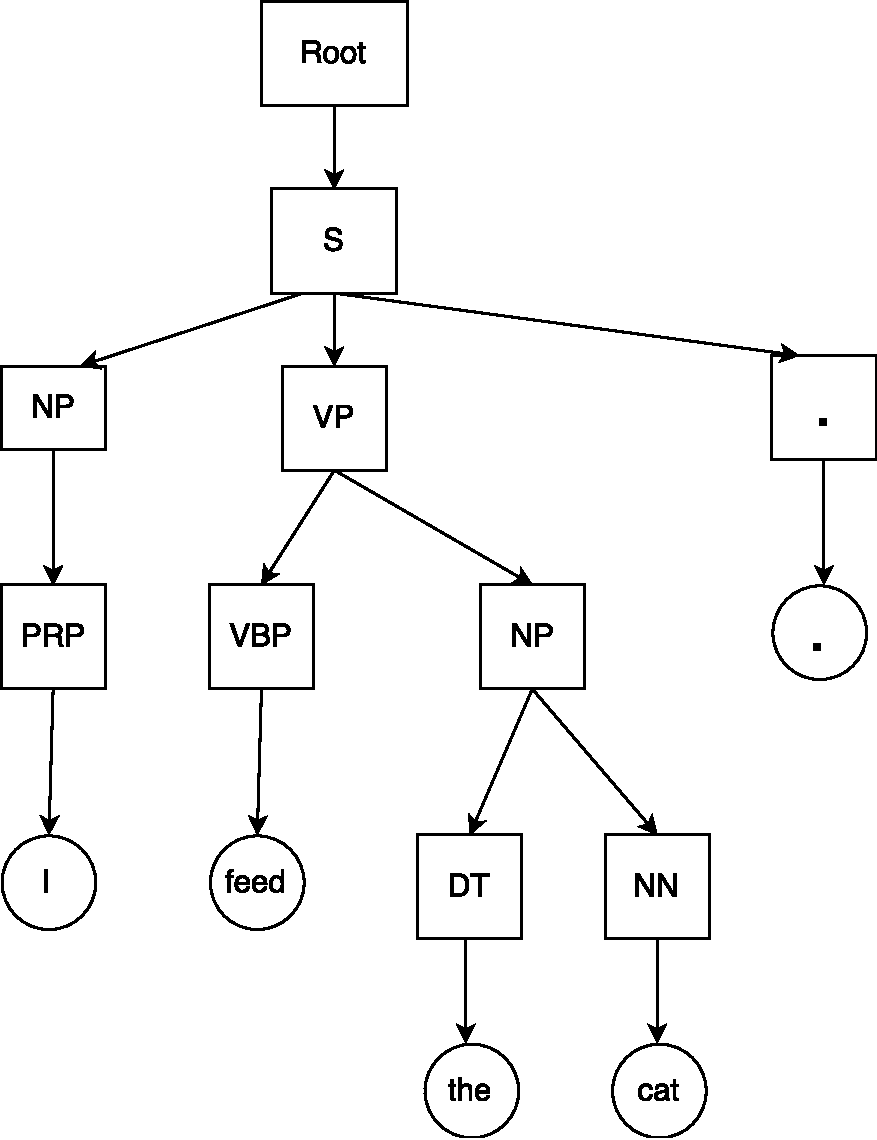
\includegraphics[width=0.5\linewidth]{figure/ifeedthecatconstituency}
    \caption[Constituency Parse Tree]{Constituency Parse Tree}
    \label{fig:ifeedthecatconstituency}
\end{figure}

\subsection{Dependency Parse Tree}
Dependency Parse Tree represents dependency relationship of each word in sentences. As oppose to Constituency Parse Tree, each node in Dependency Parse Tree contain one word. Edge are labeled by type of dependency relationship of head word and the dependent. In this thesis, we use Universal Dependencies \cite{nivre2016universal}. Fig \ref{fig:udexample} is an example of Dependency Parse Tree.

\begin{figure}[H]
    \centering
    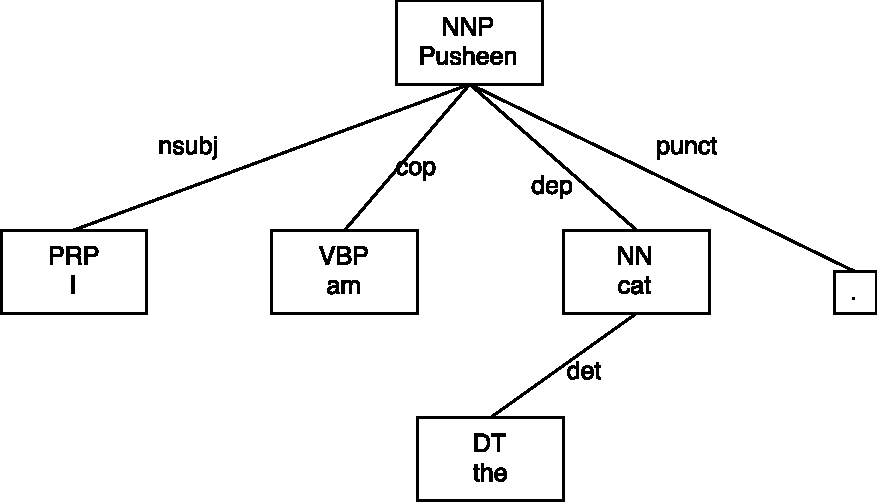
\includegraphics[width=0.7\linewidth]{figure/udexample}
    \caption[Dependency Tree]{Dependency Tree}
    \label{fig:udexample}
\end{figure}

\section{Programming Framework}
\subsection{Torch}\label{sec:torch}
Torch \footnote{http://torch.ch/} is Lua scientific computing framework. Torch support high performing matrix calculation via multi-dimensional array call Tensor. Torch is built with C/C++, CUDA backend. Torch authors chose Lua because Lua works well with C/C++ \cite{collobert2011torch7}.  Thus, Torch is high performing and support GPU. Torch have neural network package (nn) package. Computation graph must be defined before forward pass.

A simple, single linear layer network can be easily defined with few line of code (see listing \ref{lst:torchlinear}).

\begin{lstlisting}[caption={Simple linear layer in Torch},label={lst:torchlinear}, language={[5.1]Lua}]
-- simple y = Ax + b linear layer
l = nn.Linear(2,3)
-- forward pass
x = torch.Tensor(2)
y = l:forward(x) -- vector dimension of 3
\end{lstlisting}

However, when a model need multiple modules, such as multilayer perceptron (MLP), these modules must be put into container. Figure \ref{fig:nncontainer} illustrates on function of each nn container . In order to construct two-layer perception (eq \ref{eq:mlp}), linear, tanh and softmax module must be packed into sequential module (see listing \ref{lst:torchmlp}).

\begin{equation}
\label{eq:mlp}
\begin{aligned}
&h = tanh(W_1*x + b_1) \\
&y = softmax(W_2*h + b2)
\end{aligned}
\end{equation}


\begin{lstlisting}[caption={MLP in Torch},label={lst:torchmlp}, language={[5.1]Lua}]
model = nn.Sequential()
model:add(nn.Linear(2,3))
model:add(nn.Tanh())
model:add(nn.Linear(3,5))
model:add(nn.SoftMax())
-- forward
x = torch.Tensor(2)
y = model:forward(x)
\end{lstlisting}

Torch provide nngraph package support build more complicate model. For example, define MLP in (eq \ref{eq:mlp}) use nngraph (see listing \ref{lst:torchnngraph})

\begin{lstlisting}[caption={MLP using nngraph},label={lst:torchnngraph}, language={[5.1]Lua}]
model = nn.Sequential()
model:add(nn.Linear(2,3))
model:add(nn.Tanh())
model:add(nn.Linear(3,5))
model:add(nn.SoftMax())
-- forward
x = torch.Tensor(2)
y = model:forward(x)
\end{lstlisting}

Sample code on training a model, see Appendix \ref{lst:torchtrain}

\subsection{Theano}
Theano \footnote{\url{http://deeplearning.net/software/theano/}} is a deep learning library on Python. It basic function is similar to Torch: matrix calculation, support GPU. Theano is define-and-run scheme, which a computer graph must be built before it is executed.

\begin{lstlisting}[caption={Define function in Theano},label={lst:theanof}, language={python}]
x = T.dmatrix('x')
y = T.dmatrix('y')
z = x + y
f = function([x, y], z)
f([[1, 1], [2, 2]], [[3, 3], [4, 4]])
# result [[4, 4], [6, 6]]
\end{lstlisting}

Comparing to Torch7, Theano is slower on most benchmark \cite{collobert2011torch7}. Theano does not provide nice template like linear layer. Thus, model must be defined from equation. It gives researcher more control over mathematics aspect but causes more trouble for beginner. A sample code for MLP \ref{lst:theanomlp}. One more problem is that the 'define-and-run' scheme does not suitable for recursive neural network due to recompiling the computation graph each training sample take time.

\subsection{Pytorch}\label{sec:pytorch}
PyTorch uses the same backend as Torch. However, PyTorch specially designed for Python. Pytorch have pre-defined modules (Linear layer, Convolution layer) like Torch. However, Pytorch does not require to pack model into container. In Pytorch networks are defined in forward-pass thanks to Dynamic Neural Networks feature. Therefore, user can use Python control flow to define a network. For example, one can use for loop to run recurrent neural network (see listing \ref{lst:pytorchrnn}) .
This feature allows us to implement Recursive Neural Network for NLP, which the network change for every sample, much more easier. 

\begin{lstlisting}[caption={RNN},label={lst:pytorchrnn}, language={python}]
import torch
import torch.nn as nn
rnn = nn.RNNCell(10, 20)
seq_len = 10
input_dim = 100
hidden_dim = 150
input = Variable(torch.randn(seq_len, 1, input_dim))
hx = Variable(torch.zeros(1, hidden_dim))
output = []
for i in range(6):
    hx = rnn(input[i], hx)
    output.append(hx)
\end{lstlisting}

We also implement treelstm from original Torch7 \footnote{\url{https://github.com/stanfordnlp/treelstm}} sentiment classification task in PyTorch and publish on Github \footnote{\url{https://github.com/ttpro1995/TreeLSTMSentiment}}.

We choose PyTorch because:
\begin{itemize}
    \item Dynamic Neural Networks feature works well on data sequence with different length
    \item Intuitive framework
    \item Easy to install and run on CUDA
\end{itemize}
